\documentclass[border=1mm]{standalone}

\usepackage{import}
\subimport{../../../}{preamble.tex}

\usepackage{tikz}
\usetikzlibrary{calc}
\usepackage{pgfplots}



\begin{document}

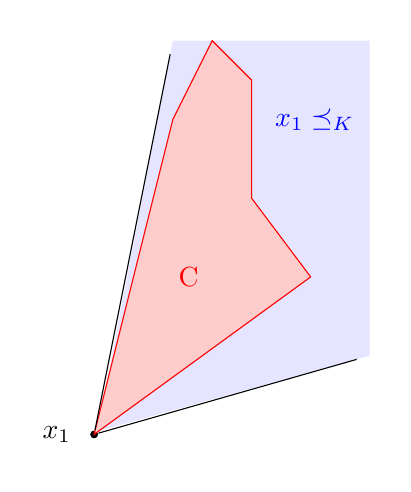
\begin{tikzpicture}[every node/.style={circle}]

  \node[fill=black, inner sep=1] at (0,0) (a) {};
  \node[left] at ($(a)-(1mm, 0mm)$) {$x_1$};
  \node at (3.5,1) (b) {};
  \node at (1,5) (c) {};


  \fill [blue!10]
  (a.north east) -- (b.center) -- (3.5, 5)  -- (c.center) -- cycle;

  \draw [draw=red, fill=red!20] (0, 0) --(1, 4) -- (1.5, 5) --(2, 4.5)--(2, 3) --(2.75, 2) -- cycle;


  \node[red] at (1.2, 2) {C};

  \node[blue] at (2.8, 4) {$x_1 \preceq_K$};
  
  \draw (a)--(b);
  \draw (a)--(c);

  
\end{tikzpicture}

\end{document}

%%% Local Variables:
%%% mode: latex
%%% TeX-master: t
%%% End:
